% Minimal DFA for the BPM response pattern  G(a -> F b), rendered directly
% from ltlf2dfa/MONA via graphviz (see gen_dfa_figs.sh). This is the canonical
% counterexample for RuleRunner's one-literal-per-subformula encoding: the DFA
% monitors the nested-temporal spec exactly, with a single canonical state
% machine that never conflates the F-b obligation spawned at each cell with the
% one still pending.
\begin{figure}[t]
  \centering
  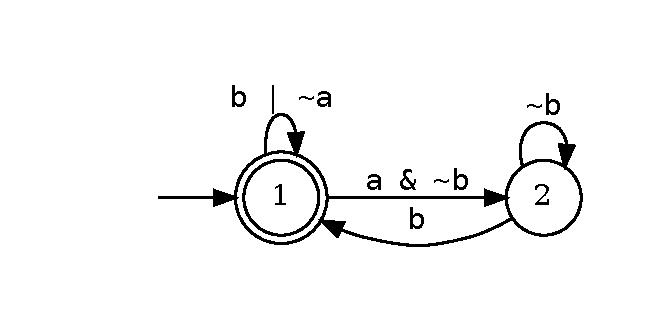
\includegraphics[width=0.55\linewidth]{fig_response_dfa.pdf}
  \caption{Minimal \DFA for the response pattern $\malways(a \limp \meventually\, b)$,
    compiled by MONA. State~$1$ (accepting) means no obligation is outstanding;
    state~$2$ means a $b$ is owed. There is no trap state and no accepting sink:
    the automaton oscillates between the two states, so no online verdict is ever
    final. A single canonical state machine tracks the outstanding obligation
    exactly, whereas RuleRunner's one-literal-per-subformula encoding conflates
    the fresh $\meventually\, b$ instance spawned at each cell with the still-pending
    one and diverges.}
  \label{fig:response-dfa}
\end{figure}
